%!TeX spellcheck = en-US
\documentclass{article}
\usepackage{enumerate}
\usepackage{amsmath}
\usepackage{amssymb}
\usepackage{graphicx}
\usepackage{subfigure}
\usepackage{geometry}
\usepackage{caption}
\usepackage{indentfirst}
\usepackage{array}
\usepackage{multicol}
%\renewcommand\arraystretch{2}
\usepackage{tikz}
\usetikzlibrary{arrows.meta}
\usepackage{multicol}
\usepackage{algorithm}
\usepackage{algorithmicx}
\usepackage{algpseudocode}
\renewcommand{\algorithmicrequire}{\textbf{Input:}}
\renewcommand{\algorithmicensure}{\textbf{Output:}}
\usepackage{minted}
\usemintedstyle{autumn}
\geometry{left=3.0 cm,right=3.0 cm,top=2.5 cm,bottom=3.0 cm}
\renewcommand{\thesection}{Ex. \arabic{section}}
\title{VE281 Writing Assignment Five}
\author{Liu Yihao 515370910207}
\date{}

\begin{document}
\maketitle

\section{}
\begin{multicols}{2}
In Kruskal's algorithm, we take the shortest edge and connect two nodes if it doesn't form a cycle.
\begin{enumerate}
	\item Connect b and c
	\item Connect a and b
	\item Connect c and e
	\item Connect e and f
	\item Connect e and d
\end{enumerate}

\columnbreak

The minimum spanning tree is
\begin{center}
  	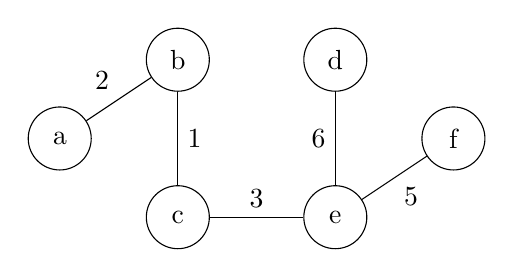
\begin{tikzpicture}
    		\draw (-2.5,0) 	node (a) [draw,shape=circle,minimum size=0.8cm] {a};
    		\draw (-1,1) 		node (b) [draw,shape=circle,minimum size=0.8cm] {b};
    		\draw (-1,-1) 	node (c) [draw,shape=circle,minimum size=0.8cm] {c};
    		\draw (1,1) 		node (d) [draw,shape=circle,minimum size=0.8cm] {d};
    		\draw (1,-1) 		node (e) [draw,shape=circle,minimum size=0.8cm] {e};
    		\draw (2.5,0) 	node (f) [draw,shape=circle,minimum size=0.8cm] {f};
    		\draw (b) edge node [right] {1} (c);
    		\draw (a) edge node [above left] {2} (b);
        \draw (c) edge node [above] {3} (e);
    		\draw (e) edge node [below right] {5} (f);
    		\draw (e) edge node [left] {6} (d);
	 \end{tikzpicture}
\end{center}

\end{multicols}

\section{}
\begin{algorithm}[H]
  	\begin{algorithmic}
    		\Require \\
    			A directed acyclic graph $G=(V,E)$ with real-valued edge weights \\
    			Two distinct nodes $s$ and $d$
    		\Ensure \\
    			A longest weighted path from $s$ to $d$ if exists \\

    		\State $L \gets G$ sorted in topological order
    		\State Remove nodes located before $s$ or after $d$ from $L$
    		\State Remove node $s$ from $L$
    		\State $s.distance \gets 0$
    		\State $s.predecessor \gets null$
    		\For {node $v$ \textbf{in} $L$}
    		    \State $v.distance \gets -\infty$
    		    \State $v.predecessor \gets null$
            \For {edge $(u,v)$ \textbf{in} edges with end node $v$}
    				    \If {$u.distance + (u,v).weight > v.distance$}
    				        \State $v.distance \gets u.distance + (u,v).weight$
                    \State $v.predecessor \gets u$
                \EndIf
    		    \EndFor
    		\EndFor
    		\If {$d.predecessor == null$}
            \State print ``No path exists"
    		\Else
    			  \State print $d.predecessor$ recursively in reverse order
    		\EndIf
  	\end{algorithmic}
\end{algorithm}

The time complexity is $O(V+E)$.

\section{}
\begin{algorithm}[H]
	\begin{algorithmic}
		\Require \\
			A directed graph $G=(V,E)$ with real-valued edge reliability in the range $[0,1]$ \\
			Two distinct nodes $s$ and $d$
		\Ensure \\
			A most reliable path from $s$ to $d$ if exists \\

		\For {node $u$ \textbf{in} $G$}
			\State $u.reached \gets false$
			\State $u.probability \gets 0$
			\State $u.predecessor \gets null$
		\EndFor
		\State $s.probability \gets 1$
		\State push node $s$ into set $S$
		\While {Set $S$ is not empty}
			\State $u \gets$ pop the node with largest reliability in $S$
			\State $u.reached \gets true$
			\For {edge $(u,v)$ \textbf{in} edges with start node $u$}
				\If {\textbf{not} $v.reached$ \textbf{and} $u.probability * (u,v).reliability > v.probability $ }
					\State $v.probability \gets u.probability * (u,v).reliability$
					\State $v.predecessor \gets u$
				\EndIf
			\EndFor
		\EndWhile

		\If {$d.predecessor == null$}
			\State print ``No path exists"
		\Else
			\State print $d.predecessor$ recursively in reverse order
		\EndIf
	\end{algorithmic}
\end{algorithm}

\section{}
\begin{algorithm}[H]
	\begin{algorithmic}
		\Require \\
			A connected, undirected graph $G=(V,E)$
		\Ensure \\
			A path that traverses edge in E exactly once in each direction. \\

		\For {node $u$ \textbf{in} $G$}
			\State $u.reached \gets false$
			\State $u.depth \gets 0$
		\EndFor
		\State $s \gets$ an arbitrary node in $G$
		\State \Call {DFS}{$s$}
		\\
		\Function {DFS}{node $u$}
			\State $u.reached \gets true$
			\For {edge $(u,v)$ \textbf{in} edges adjacent to $u$}
				\If {\textbf{not} $v.reached$}
					\State $v.depth \gets u.depth + 1$
					\State traverse $u \to v$
					\State \Call {DFS}{$v$}
					\State traverse $v \to u$
				\ElsIf {$v.depth > u.depth$}
					\State traverse $u \to v$
					\State traverse $v \to u$
				\EndIf
			\EndFor
		\EndFunction

	\end{algorithmic}
\end{algorithm}

\section{}

\begin{multicols}{2}
\noindent Iteration 1\\
Edge a -> b = 6\\
a: distance = 0, predecessor = null\\
b: distance = inf, predecessor = null\\
updated: b: distance = 6, predecessor = a\\
Edge a -> c = 4\\
a: distance = 0, predecessor = null\\
c: distance = inf, predecessor = null\\
updated: c: distance = 4, predecessor = a\\
Edge b -> c = 1\\
b: distance = 6, predecessor = a\\
c: distance = 4, predecessor = a\\
nothing happened\\
Edge b -> d = 5\\
b: distance = 6, predecessor = a\\
d: distance = inf, predecessor = null\\
updated: d: distance = 11, predecessor = b\\
Edge b -> f = 6\\
b: distance = 6, predecessor = a\\
f: distance = inf, predecessor = null\\
updated: f: distance = 12, predecessor = b\\
Edge c -> e = 3\\
c: distance = 4, predecessor = a\\
e: distance = inf, predecessor = null\\
updated: e: distance = 7, predecessor = c\\
Edge d -> e = 1\\
d: distance = 11, predecessor = b\\
e: distance = 7, predecessor = c\\
nothing happened\\
Edge e -> b = -2\\
e: distance = 7, predecessor = c\\
b: distance = 6, predecessor = a\\
updated: b: distance = 5, predecessor = e\\
Edge e -> f = 6\\
e: distance = 7, predecessor = c\\
f: distance = 12, predecessor = b\\
nothing happened\\
Edge f -> d = -3\\
f: distance = 12, predecessor = b\\
d: distance = 11, predecessor = b\\
updated: d: distance = 9, predecessor = f\\

\begin{center}
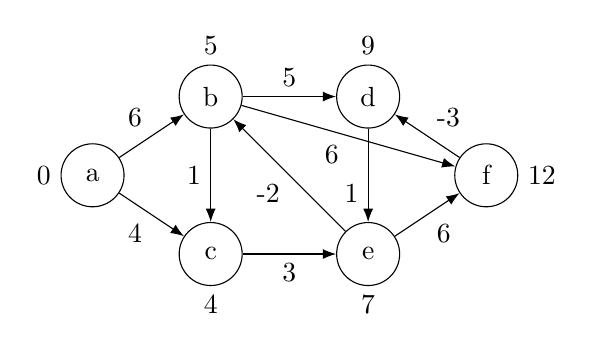
\begin{tikzpicture}[>/.tip={Latex}]
\draw (-2.5,0) 	node (a) [draw,shape=circle,minimum size=0.8cm] {a};
\draw (-1,1)    node (b) [draw,shape=circle,minimum size=0.8cm] {b};
\draw (-1,-1)   node (c) [draw,shape=circle,minimum size=0.8cm] {c};
\draw (1,1)     node (d) [draw,shape=circle,minimum size=0.8cm] {d};
\draw (1,-1)    node (e) [draw,shape=circle,minimum size=0.8cm] {e};
\draw (2.5,0)   node (f) [draw,shape=circle,minimum size=0.8cm] {f};
\draw[->] (a) edge node [above left] {6} (b);
\draw[->] (a) edge node [below left] {4} (c);
\draw[->] (b) edge node [left] {1} (c);
\draw[->] (b) edge node [above] {5} (d);
\draw[->] (b) edge node [below left] {6} (f);
\draw[->] (c) edge node [below] {3} (e);
\draw[->] (d) edge node [below left] {1} (e);
\draw[->] (e) edge node [below left] {-2} (b);
\draw[->] (e) edge node [below right] {6} (f);
\draw[->] (f) edge node [above right] {-3} (d);
    
\node [left]  at (a.west)  {0};
\node [above] at (b.north) {5};
\node [below] at (c.south) {4};
\node [above] at (d.north) {9};
\node [below] at (e.south) {7};
\node [right] at (f.east)  {12};

\end{tikzpicture}
\end{center}
    
\noindent Iteration 2\\
Edge a -> b = 6\\
a: distance = 0, predecessor = null\\
b: distance = 5, predecessor = e\\
nothing happened\\
Edge a -> c = 4\\
a: distance = 0, predecessor = null\\
c: distance = 4, predecessor = a\\
nothing happened\\
Edge b -> c = 1\\
b: distance = 5, predecessor = e\\
c: distance = 4, predecessor = a\\
nothing happened\\
Edge b -> d = 5\\
b: distance = 5, predecessor = e\\
d: distance = 9, predecessor = f\\
nothing happened\\
Edge b -> f = 6\\
b: distance = 5, predecessor = e\\
f: distance = 12, predecessor = b\\
updated: f: distance = 11, predecessor = b\\
Edge c -> e = 3\\
c: distance = 4, predecessor = a\\
e: distance = 7, predecessor = c\\
nothing happened\\
Edge d -> e = 1\\
d: distance = 9, predecessor = f\\
e: distance = 7, predecessor = c\\
nothing happened\\
Edge e -> b = -2\\
e: distance = 7, predecessor = c\\
b: distance = 5, predecessor = e\\
nothing happened\\
Edge e -> f = 6\\
e: distance = 7, predecessor = c\\
f: distance = 11, predecessor = b\\
nothing happened\\
Edge f -> d = -3\\
f: distance = 11, predecessor = b\\
d: distance = 9, predecessor = f\\
updated: d: distance = 8, predecessor = f\\

\begin{center}
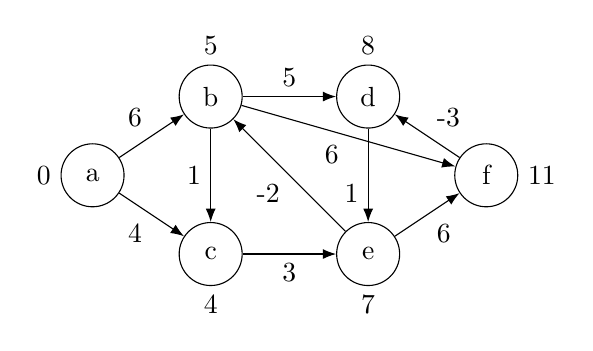
\begin{tikzpicture}[>/.tip={Latex}]
\draw (-2.5,0) 	node (a) [draw,shape=circle,minimum size=0.8cm] {a};
\draw (-1,1)    node (b) [draw,shape=circle,minimum size=0.8cm] {b};
\draw (-1,-1)   node (c) [draw,shape=circle,minimum size=0.8cm] {c};
\draw (1,1)     node (d) [draw,shape=circle,minimum size=0.8cm] {d};
\draw (1,-1)    node (e) [draw,shape=circle,minimum size=0.8cm] {e};
\draw (2.5,0)   node (f) [draw,shape=circle,minimum size=0.8cm] {f};
\draw[->] (a) edge node [above left] {6} (b);
\draw[->] (a) edge node [below left] {4} (c);
\draw[->] (b) edge node [left] {1} (c);
\draw[->] (b) edge node [above] {5} (d);
\draw[->] (b) edge node [below left] {6} (f);
\draw[->] (c) edge node [below] {3} (e);
\draw[->] (d) edge node [below left] {1} (e);
\draw[->] (e) edge node [below left] {-2} (b);
\draw[->] (e) edge node [below right] {6} (f);
\draw[->] (f) edge node [above right] {-3} (d);
    
\node [left]  at (a.west)  {0};
\node [above] at (b.north) {5};
\node [below] at (c.south) {4};
\node [above] at (d.north) {8};
\node [below] at (e.south) {7};
\node [right] at (f.east)  {11};

\end{tikzpicture}
\end{center}
    
\noindent Iteration 3\\
Edge a -> b = 6\\
a: distance = 0, predecessor = null\\
b: distance = 5, predecessor = e\\
nothing happened\\
Edge a -> c = 4\\
a: distance = 0, predecessor = null\\
c: distance = 4, predecessor = a\\
nothing happened\\
Edge b -> c = 1\\
b: distance = 5, predecessor = e\\
c: distance = 4, predecessor = a\\
nothing happened\\
Edge b -> d = 5\\
b: distance = 5, predecessor = e\\
d: distance = 8, predecessor = f\\
nothing happened\\
Edge b -> f = 6\\
b: distance = 5, predecessor = e\\
f: distance = 11, predecessor = b\\
nothing happened\\
Edge c -> e = 3\\
c: distance = 4, predecessor = a\\
e: distance = 7, predecessor = c\\
nothing happened\\
Edge d -> e = 1\\
d: distance = 8, predecessor = f\\
e: distance = 7, predecessor = c\\
nothing happened\\
Edge e -> b = -2\\
e: distance = 7, predecessor = c\\
b: distance = 5, predecessor = e\\
nothing happened\\
Edge e -> f = 6\\
e: distance = 7, predecessor = c\\
f: distance = 11, predecessor = b\\
nothing happened\\
Edge f -> d = -3\\
f: distance = 11, predecessor = b\\
d: distance = 8, predecessor = f\\
nothing happened\\

\begin{center}
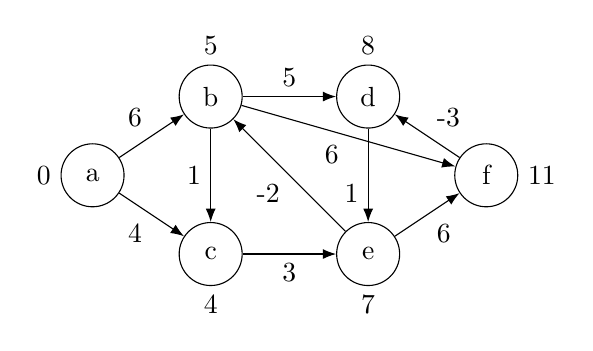
\begin{tikzpicture}[>/.tip={Latex}]
\draw (-2.5,0) 	node (a) [draw,shape=circle,minimum size=0.8cm] {a};
\draw (-1,1)    node (b) [draw,shape=circle,minimum size=0.8cm] {b};
\draw (-1,-1)   node (c) [draw,shape=circle,minimum size=0.8cm] {c};
\draw (1,1)     node (d) [draw,shape=circle,minimum size=0.8cm] {d};
\draw (1,-1)    node (e) [draw,shape=circle,minimum size=0.8cm] {e};
\draw (2.5,0)   node (f) [draw,shape=circle,minimum size=0.8cm] {f};
\draw[->] (a) edge node [above left] {6} (b);
\draw[->] (a) edge node [below left] {4} (c);
\draw[->] (b) edge node [left] {1} (c);
\draw[->] (b) edge node [above] {5} (d);
\draw[->] (b) edge node [below left] {6} (f);
\draw[->] (c) edge node [below] {3} (e);
\draw[->] (d) edge node [below left] {1} (e);
\draw[->] (e) edge node [below left] {-2} (b);
\draw[->] (e) edge node [below right] {6} (f);
\draw[->] (f) edge node [above right] {-3} (d);
    
\node [left]  at (a.west)  {0};
\node [above] at (b.north) {5};
\node [below] at (c.south) {4};
\node [above] at (d.north) {8};
\node [below] at (e.south) {7};
\node [right] at (f.east)  {11};

\end{tikzpicture}
\end{center}
    
\noindent Iteration 4\\
Edge a -> b = 6\\
a: distance = 0, predecessor = null\\
b: distance = 5, predecessor = e\\
nothing happened\\
Edge a -> c = 4\\
a: distance = 0, predecessor = null\\
c: distance = 4, predecessor = a\\
nothing happened\\
Edge b -> c = 1\\
b: distance = 5, predecessor = e\\
c: distance = 4, predecessor = a\\
nothing happened\\
Edge b -> d = 5\\
b: distance = 5, predecessor = e\\
d: distance = 8, predecessor = f\\
nothing happened\\
Edge b -> f = 6\\
b: distance = 5, predecessor = e\\
f: distance = 11, predecessor = b\\
nothing happened\\
Edge c -> e = 3\\
c: distance = 4, predecessor = a\\
e: distance = 7, predecessor = c\\
nothing happened\\
Edge d -> e = 1\\
d: distance = 8, predecessor = f\\
e: distance = 7, predecessor = c\\
nothing happened\\
Edge e -> b = -2\\
e: distance = 7, predecessor = c\\
b: distance = 5, predecessor = e\\
nothing happened\\
Edge e -> f = 6\\
e: distance = 7, predecessor = c\\
f: distance = 11, predecessor = b\\
nothing happened\\
Edge f -> d = -3\\
f: distance = 11, predecessor = b\\
d: distance = 8, predecessor = f\\
nothing happened\\

\begin{center}
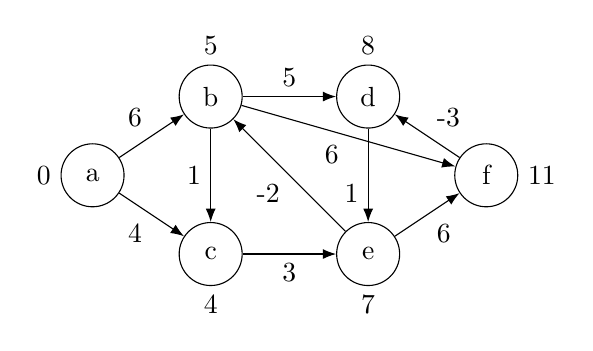
\begin{tikzpicture}[>/.tip={Latex}]
\draw (-2.5,0) 	node (a) [draw,shape=circle,minimum size=0.8cm] {a};
\draw (-1,1)    node (b) [draw,shape=circle,minimum size=0.8cm] {b};
\draw (-1,-1)   node (c) [draw,shape=circle,minimum size=0.8cm] {c};
\draw (1,1)     node (d) [draw,shape=circle,minimum size=0.8cm] {d};
\draw (1,-1)    node (e) [draw,shape=circle,minimum size=0.8cm] {e};
\draw (2.5,0)   node (f) [draw,shape=circle,minimum size=0.8cm] {f};
\draw[->] (a) edge node [above left] {6} (b);
\draw[->] (a) edge node [below left] {4} (c);
\draw[->] (b) edge node [left] {1} (c);
\draw[->] (b) edge node [above] {5} (d);
\draw[->] (b) edge node [below left] {6} (f);
\draw[->] (c) edge node [below] {3} (e);
\draw[->] (d) edge node [below left] {1} (e);
\draw[->] (e) edge node [below left] {-2} (b);
\draw[->] (e) edge node [below right] {6} (f);
\draw[->] (f) edge node [above right] {-3} (d);
    
\node [left]  at (a.west)  {0};
\node [above] at (b.north) {5};
\node [below] at (c.south) {4};
\node [above] at (d.north) {8};
\node [below] at (e.south) {7};
\node [right] at (f.east)  {11};

\end{tikzpicture}
\end{center}
    
\noindent Iteration 5\\
Edge a -> b = 6\\
a: distance = 0, predecessor = null\\
b: distance = 5, predecessor = e\\
nothing happened\\
Edge a -> c = 4\\
a: distance = 0, predecessor = null\\
c: distance = 4, predecessor = a\\
nothing happened\\
Edge b -> c = 1\\
b: distance = 5, predecessor = e\\
c: distance = 4, predecessor = a\\
nothing happened\\
Edge b -> d = 5\\
b: distance = 5, predecessor = e\\
d: distance = 8, predecessor = f\\
nothing happened\\
Edge b -> f = 6\\
b: distance = 5, predecessor = e\\
f: distance = 11, predecessor = b\\
nothing happened\\
Edge c -> e = 3\\
c: distance = 4, predecessor = a\\
e: distance = 7, predecessor = c\\
nothing happened\\
Edge d -> e = 1\\
d: distance = 8, predecessor = f\\
e: distance = 7, predecessor = c\\
nothing happened\\
Edge e -> b = -2\\
e: distance = 7, predecessor = c\\
b: distance = 5, predecessor = e\\
nothing happened\\
Edge e -> f = 6\\
e: distance = 7, predecessor = c\\
f: distance = 11, predecessor = b\\
nothing happened\\
Edge f -> d = -3\\
f: distance = 11, predecessor = b\\
d: distance = 8, predecessor = f\\
nothing happened\\

\begin{center}
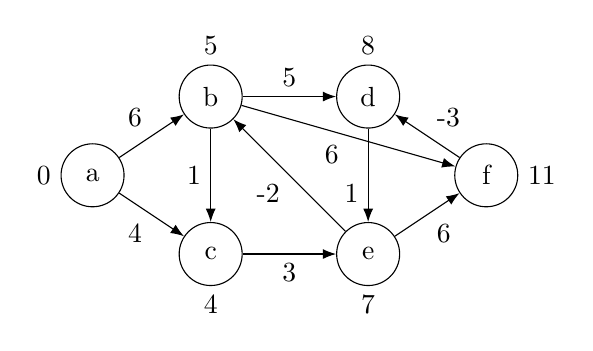
\begin{tikzpicture}[>/.tip={Latex}]
\draw (-2.5,0) 	node (a) [draw,shape=circle,minimum size=0.8cm] {a};
\draw (-1,1)    node (b) [draw,shape=circle,minimum size=0.8cm] {b};
\draw (-1,-1)   node (c) [draw,shape=circle,minimum size=0.8cm] {c};
\draw (1,1)     node (d) [draw,shape=circle,minimum size=0.8cm] {d};
\draw (1,-1)    node (e) [draw,shape=circle,minimum size=0.8cm] {e};
\draw (2.5,0)   node (f) [draw,shape=circle,minimum size=0.8cm] {f};
\draw[->] (a) edge node [above left] {6} (b);
\draw[->] (a) edge node [below left] {4} (c);
\draw[->] (b) edge node [left] {1} (c);
\draw[->] (b) edge node [above] {5} (d);
\draw[->] (b) edge node [below left] {6} (f);
\draw[->] (c) edge node [below] {3} (e);
\draw[->] (d) edge node [below left] {1} (e);
\draw[->] (e) edge node [below left] {-2} (b);
\draw[->] (e) edge node [below right] {6} (f);
\draw[->] (f) edge node [above right] {-3} (d);
    
\node [left]  at (a.west)  {0};
\node [above] at (b.north) {5};
\node [below] at (c.south) {4};
\node [above] at (d.north) {8};
\node [below] at (e.south) {7};
\node [right] at (f.east)  {11};

\end{tikzpicture}
\end{center}
    
\noindent Iteration 6\\
Edge a -> b = 6\\
a: distance = 0, predecessor = null\\
b: distance = 5, predecessor = e\\
nothing happened\\
Edge a -> c = 4\\
a: distance = 0, predecessor = null\\
c: distance = 4, predecessor = a\\
nothing happened\\
Edge b -> c = 1\\
b: distance = 5, predecessor = e\\
c: distance = 4, predecessor = a\\
nothing happened\\
Edge b -> d = 5\\
b: distance = 5, predecessor = e\\
d: distance = 8, predecessor = f\\
nothing happened\\
Edge b -> f = 6\\
b: distance = 5, predecessor = e\\
f: distance = 11, predecessor = b\\
nothing happened\\
Edge c -> e = 3\\
c: distance = 4, predecessor = a\\
e: distance = 7, predecessor = c\\
nothing happened\\
Edge d -> e = 1\\
d: distance = 8, predecessor = f\\
e: distance = 7, predecessor = c\\
nothing happened\\
Edge e -> b = -2\\
e: distance = 7, predecessor = c\\
b: distance = 5, predecessor = e\\
nothing happened\\
Edge e -> f = 6\\
e: distance = 7, predecessor = c\\
f: distance = 11, predecessor = b\\
nothing happened\\
Edge f -> d = -3\\
f: distance = 11, predecessor = b\\
d: distance = 8, predecessor = f\\
nothing happened\\

\begin{center}
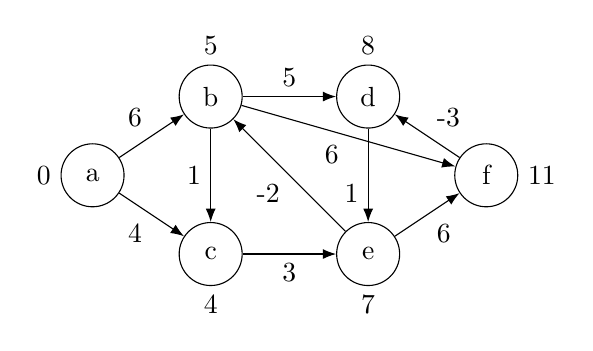
\begin{tikzpicture}[>/.tip={Latex}]
\draw (-2.5,0) 	node (a) [draw,shape=circle,minimum size=0.8cm] {a};
\draw (-1,1)    node (b) [draw,shape=circle,minimum size=0.8cm] {b};
\draw (-1,-1)   node (c) [draw,shape=circle,minimum size=0.8cm] {c};
\draw (1,1)     node (d) [draw,shape=circle,minimum size=0.8cm] {d};
\draw (1,-1)    node (e) [draw,shape=circle,minimum size=0.8cm] {e};
\draw (2.5,0)   node (f) [draw,shape=circle,minimum size=0.8cm] {f};
\draw[->] (a) edge node [above left] {6} (b);
\draw[->] (a) edge node [below left] {4} (c);
\draw[->] (b) edge node [left] {1} (c);
\draw[->] (b) edge node [above] {5} (d);
\draw[->] (b) edge node [below left] {6} (f);
\draw[->] (c) edge node [below] {3} (e);
\draw[->] (d) edge node [below left] {1} (e);
\draw[->] (e) edge node [below left] {-2} (b);
\draw[->] (e) edge node [below right] {6} (f);
\draw[->] (f) edge node [above right] {-3} (d);
    
\node [left]  at (a.west)  {0};
\node [above] at (b.north) {5};
\node [below] at (c.south) {4};
\node [above] at (d.north) {8};
\node [below] at (e.south) {7};
\node [right] at (f.east)  {11};

\end{tikzpicture}
\end{center}
    
\noindent Check negative cycle\\
Edge a -> b = 6\\
a: distance = 0, predecessor = null\\
b: distance = 5, predecessor = e\\
nothing happened\\
Edge a -> c = 4\\
a: distance = 0, predecessor = null\\
c: distance = 4, predecessor = a\\
nothing happened\\
Edge b -> c = 1\\
b: distance = 5, predecessor = e\\
c: distance = 4, predecessor = a\\
nothing happened\\
Edge b -> d = 5\\
b: distance = 5, predecessor = e\\
d: distance = 8, predecessor = f\\
nothing happened\\
Edge b -> f = 6\\
b: distance = 5, predecessor = e\\
f: distance = 11, predecessor = b\\
nothing happened\\
Edge c -> e = 3\\
c: distance = 4, predecessor = a\\
e: distance = 7, predecessor = c\\
nothing happened\\
Edge d -> e = 1\\
d: distance = 8, predecessor = f\\
e: distance = 7, predecessor = c\\
nothing happened\\
Edge e -> b = -2\\
e: distance = 7, predecessor = c\\
b: distance = 5, predecessor = e\\
nothing happened\\
Edge e -> f = 6\\
e: distance = 7, predecessor = c\\
f: distance = 11, predecessor = b\\
nothing happened\\
Edge f -> d = -3\\
f: distance = 11, predecessor = b\\
d: distance = 8, predecessor = f\\
nothing happened\\

\noindent Graph doesn't contain a negative-weight cycle

\end{multicols}

\section{}
According to the algorithm, if $L(v, j)$ doesn't change in one iteration, then in the next iteration, since the initial condition and order are the same, $L(v, j+1)$ won't change as well. So when the iteration is completed, the value of $L(v, |V|)$ equals to $L(v, j)$, and in the procedure of checking negative cycles, $L(v, |V|+1)$ also doesn't change. So I can stop and claim that there is no negative cycle and the length of the shortest $s-v$ path is $L(v, j)$ for all $v \in V $.

\section{}

In the main loop, there are two loops, which have time complexity $O(n^2)$. And when we want to find $\min\limits_{1\leqslant k\leqslant i-1}\{s[k][i-1]\}$, iterating from $i-1$ down to 1, if $s[k_0][i-1]=+\infty$, we can claim that for all $k<k_0$, $s[k_0][i-1]=+\infty$, so the loop can be break. And we know that at most $M/2$ words are on one line, so this iteration have at most $M/2$ times. Since $M$ is a constant in the problem, the overall time complexity is $O(n^2)$.

\begin{algorithm}[H]
	\begin{algorithmic}
		\Require \\
			A sequence of $n$ words of lengths $l_1,l_2,\cdots,l_n$
		\Ensure \\
			Print a paragraph of $n$ words neatly so that the sum of cubes of extra space is minimum

		\For {$i \gets 1$ \textbf{to} $n$}
        \State $sum \gets 0$
        \For {$j \gets i$ \textbf{to} $n$}
            \State $sum \gets sum + l_j$
            \State $space \gets M - j + i - sum$
            \If {$space >= 0$}
                \State $v[i][j] \gets space * space * space$
            \Else
                \State $v[i][j] \gets +\infty$
            \EndIf
        \EndFor
        \If {$v[i][n] != +\infty$}
            \State $v[i][n] \gets 0$
        \EndIf
		\EndFor

    \For {$i \gets 1$ \textbf{to} $n$}
        \State $s[0][i] \gets v[0][i]$
    \EndFor

    \For {$j \gets 2$ \textbf{to} $n$}
        \For {$i \gets j$ \textbf{downto} $2$}
            \If {$v[i][j] == +\infty$}
                \State \textbf{break}
            \EndIf
            \State $value \gets \min\limits_{1\leqslant k\leqslant i-1}\{s[k][i-1]\}, index \gets k$
            \State $s[i][j] \gets v[i][j] + value$
            \State $p[i][j] \gets index$
        \EndFor
    \EndFor

    \State $min \gets \min\limits_{1\leqslant i\leqslant i-1}\{s[i][n]\}, begin \gets i$
    \State $end \gets n$
    \While {$begin>0$}
        \State prepends $\{begin,end\}$ to $list$
        \State $temp \gets begin$
        \State $begin \gets p[begin][end]$
        \State $end \gets temp - 1$
    \EndWhile
    \State prepends $\{begin,end\}$ to $list$
	\For {$\{begin,end\}$ \textbf{in} $list$}
		\State print words between $begin$ and $end$, ended with a new line
	\EndFor	
	\end{algorithmic}
\end{algorithm}



\end{document}
